\documentclass[12pt,oneside]{book}

\usepackage{geometry}                
\geometry{a4paper}                   		 
%\geometry{landscape}                		% Activate for for rotated page geometry
%\usepackage[parfill]{parskip}    		% Activate to begin paragraphs with an empty line rather than an indent
\usepackage{graphicx}				% Use pdf, png, jpg, or epsß with pdflatex; use eps in DVI mode
								% TeX will automatically convert eps --> pdf in pdflatex		
\usepackage{amssymb}
\usepackage{color}

\usepackage[spanish]{babel}			% Permite que partes automáticas del documento aparezcan en castellano.
\usepackage[utf8]{inputenc}			% Permite escribir tildes y otros caracteres directamente en el .tex
\usepackage[T1]{fontenc}				% Asegura que el documento resultante use caracteres de una fuente apropiada.

\usepackage{hyperref}				% Permite poner urls y links dentro del documento

\title{Mi Juego Favorito}
\author{Dennise Pintado \\ Keyla Figueroa \\ Agusto Ortiz}
%\date{}							% Activate to display a given date or no date

\begin{document}
\maketitle
\tableofcontents

\chapter{Introducción}
En este documento se encuentran los juegos favoritos de los integrantes de este grupo, juegos que se han destacado por sus gráficos y por su gran calidad de contenido.

\chapter{Mis Juegos Preferidos}
\section{Mario Kart 64}

\begin{figure}[htbp]
\begin{center}
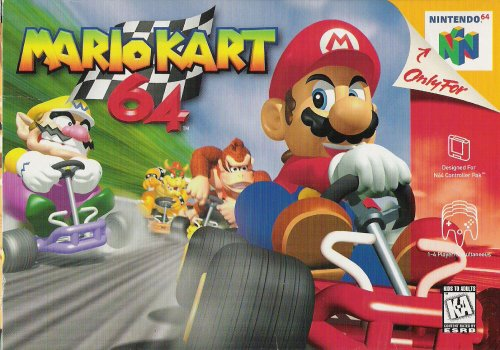
\includegraphics[width=.60\textwidth]{./imagenes/kart1.jpg} 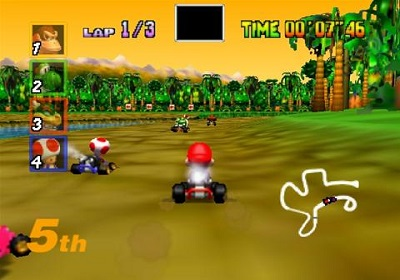
\includegraphics[width=.60\textwidth]{./imagenes/kart2.jpg} 
\caption{MarioKart}
\label{Mario Kart}
\end{center}
\end{figure}

\begin{itemize}
\item[Dennise Pintado] Ahora en un mundo donde el poder computacional de las maquinas hacen que todos deseemos  gráficos cada vez más realistas, nos encontramos con gustos algo antiguos u obsoletos pero a mi parecer es como las películas o músicas clásicas, nunca pasaran de moda. Cuando mis padres compraron la consola del Nintendo 64 el primer juego a probar fue el MarioKart 64,  con  64 bits de potencia gráfica la inmersión producida en el juego  por estos gráficos 3D llenos de colores, combinado con la iluminación de las carreteras en las que se corría, los efectos de sonido de cada estrella, cascaron, bananas  y el vibrar del control de mando cuando topaba con alguna de estas, me hacían sentir una experiencia de usuario fantástica. Con sus cuatro entradas se podían disfrutar de experiencias multijugador y el  control del juego que se tenía con este  mando era único, ya que su diseño era totalmente adaptable a la mano y daba un control de 360 grados alrededor de la escena que se jugaba.  
\end{itemize}



\chapter{Conclusiones}
Cuales juegos fueron más populares y un breve razonamiento del porqué.

\end{document}  